\documentclass[crop,border=7pt]{standalone}
\usepackage{tikz}
\usepackage{ifthen}
\usetikzlibrary{shapes.geometric}
\tikzset{
  hexagone/.style={
    draw, thick,
    fill=blue!20,
    shape=regular polygon,
    regular polygon sides=6,
    outer sep=0, inner sep=0,
    minimum size=1cm,
    %label={[red]center:#1}
  }
}
\begin{document}
  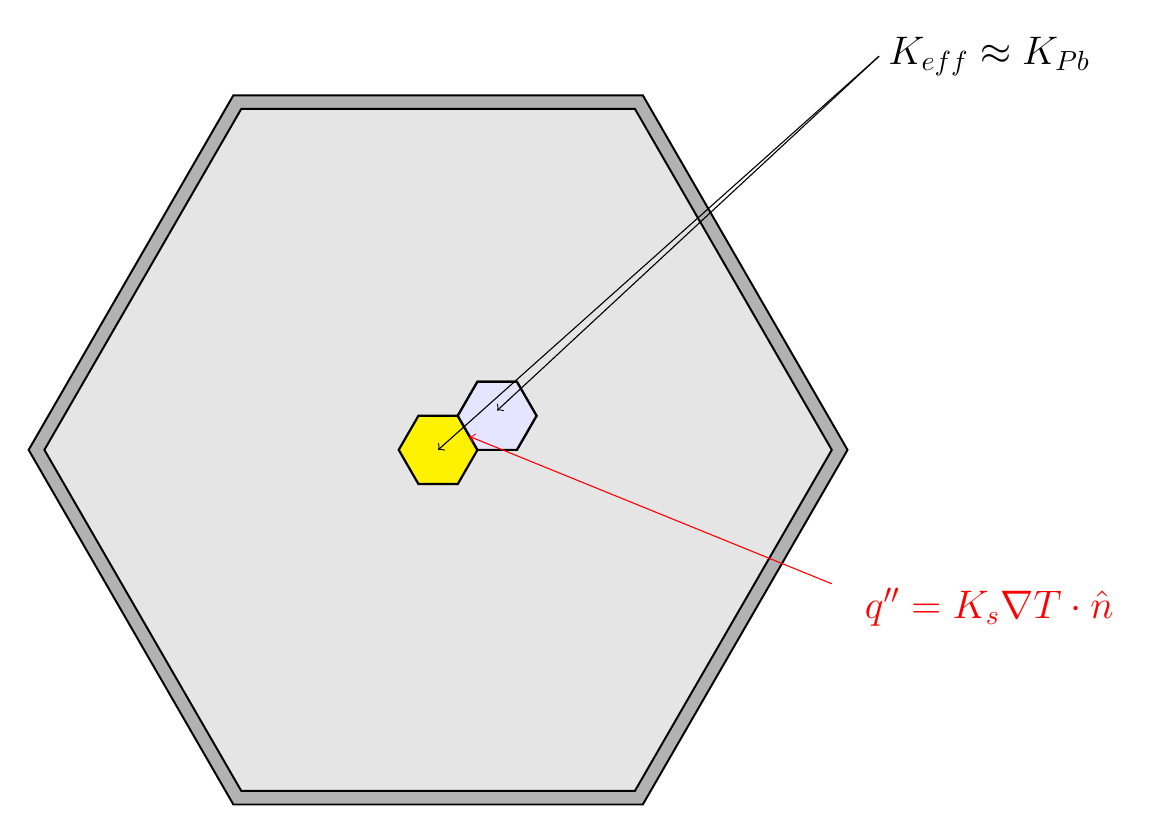
\begin{tikzpicture}
  
\newdimen\R
\R=5.2cm
  \coordinate (center) at (0,0);
 \filldraw[gray!60, draw=black,line width=0.25mm] (0:\R)
     \foreach \x in {60,120,...,360} {  -- (\x:\R) }
              -- cycle (300:\R)
              -- cycle (240:\R) 
              -- cycle (180:\R) 
              -- cycle (120:\R) 
              -- cycle (60:\R) 
              -- cycle (0:\R) ;
%%%%%%%%%
%%%hexagon 2
\newdimen\R
\R=5cm
  \coordinate (center) at (0,0);
   \filldraw[gray!20, draw=black,line width=0.25mm] (0:\R)
     \foreach \x in {60,120,...,360} {  -- (\x:\R) }
              -- cycle (300:\R)
              -- cycle (240:\R) 
              -- cycle (180:\R) 
              -- cycle (120:\R) 
              -- cycle (60:\R) 
              -- cycle (0:\R) ;
              
%%%%%%%%%firstloop circle
    \node[hexagone=0, fill=yellow ] at (0,0){};
    \foreach \r in {1,...,1}
      \foreach \t in {0,...,1}
        \foreach[evaluate={\l=int(\r*(\r-1)*3+\r*\t+\u)}] \u in {1,...,\r}
            \node[hexagone=\l, fill=blue!10] at (0+.75*\u,{0.43301270189*(2*\r-\u)}){};
            
            
            
            
    \draw [->] (5.6,5) -- (0,0);
    \draw [->] (5.6,5) -- (0.75,0.5);
    \node [align=right] at (7,5) {\Large $K_{eff}\approx K_{Pb}$};
    
    \draw [red,->] (5,-1.7) -- (0.4,0.17);
    \node [align=right] at (7,-2) {\Large \textcolor{red}{$q''=K_s \nabla T \cdot \hat{n}$}};
            
            

   
   
   
   
    %Legend
%         \node[anchor=east] at (-9,-6) (leg1) {$1$. PSU};
%         \node[below=1mm of leg1] (leg2) {$2$. Sputter Source};
%         \node[right=6mm of leg1,anchor=west] (leg8) {$8$. Pumps};

%%LEGEND
%\draw (7,5.5) rectangle (12,10);
%\matrix [below left] at (current bounding box.north east) {
%  \node [bluenode, label=right:\LARGE In-Pile Section] {}; \\  
%  \node [violetnode, label=right:\LARGE Safety Rod] {}; \\
%  \node [yellownode, label=right:\LARGE Inner MOX Fuel] {}; \\
%  \node [rednode, label=right:\LARGE Outer MOX Fuel ] {}; \\
%  \node [greennode, label=right:\LARGE Control Rod] {}; \\  
%  \node [graynode, label=right:\LARGE Dummy Section] {}; \\  
%};

  \end{tikzpicture}
\end{document}